% =============================================================================
% Dídac Llorens — shared CV preamble
% Shared only: packages, layout, reusable components, stable candidate data,
% generic metadata defaults, header, common background and common education.
% Role-specific CV files should contain only \cvsetup{...} plus visible content.
% =============================================================================

\usepackage[utf8]{inputenc}
\usepackage[T1]{fontenc}
\usepackage[english]{babel}

\usepackage[
  a4paper,
  top=0.90cm,
  bottom=0.90cm,
  left=1.00cm,
  right=1.00cm
]{geometry}

\usepackage{graphicx}
\usepackage{array}
\usepackage{tabularx}
\usepackage{enumitem}
\usepackage{xcolor}
\usepackage{transparent}

\definecolor{ink}{HTML}{111827}
\definecolor{muted}{HTML}{4B5563}
\definecolor{soft}{HTML}{F3F4F6}
\definecolor{line}{HTML}{D1D5DB}
\definecolor{linkblue}{HTML}{1D4ED8}
\definecolor{accent}{HTML}{0F172A}

\usepackage[
  unicode=true,
  pdfencoding=auto,
  colorlinks=true,
  linkcolor=accent,
  urlcolor=linkblue
]{hyperref}

\pagestyle{empty}
\raggedbottom
\urlstyle{same}
\setlength{\parindent}{0pt}
\setlength{\parskip}{0.12em}
\renewcommand{\arraystretch}{1.01}
\setlist[itemize]{leftmargin=1.05em,itemsep=0.03em,topsep=0.05em,parsep=0em}

\newlength{\RailWidth}
\newlength{\MainWidth}
\newlength{\BodyHeight}
\setlength{\RailWidth}{0.25\textwidth}
\setlength{\MainWidth}{0.70\textwidth}
\setlength{\BodyHeight}{0.835\textheight}

\newcolumntype{Y}{>{\raggedright\arraybackslash}X}
\newcolumntype{L}[1]{>{\raggedright\arraybackslash\hyphenpenalty=10000\exhyphenpenalty=10000}p{#1}}

% -----------------------------------------------------------------------------
% Reusable visual components
% -----------------------------------------------------------------------------

\newcommand{\sep}{\textcolor{line}{\quad|\quad}}

% Avoid \tag: it commonly collides with other LaTeX packages/templates.
\newcommand{\cvpill}[1]{%
  \scriptsize\colorbox{soft}{\strut\hspace{0.22em}#1\hspace{0.22em}}%
}

\newcommand{\mainsection}[1]{%
  \vspace{1.30em}%
  {\hspace*{\fill}\large\bfseries\ttfamily\color{accent}#1~~}\par
  \vspace{0.3em}%
  {\color{line}\hrule}%
  \vspace{0.5em}%
}

\newcommand{\railsection}[1]{%
  \vspace{3em}%
  {\large\bfseries\ttfamily\MakeUppercase{#1}}\par
  \vspace{0.7em}%
  {\color{line}\hrule}%
  \vspace{0.7em}%
}

\newcommand{\project}[4]{%
  {\bfseries #1}\hfill{\scriptsize\textcolor{muted}{#2}}\par
  #3\par
  {\scriptsize #4}\par
  \vspace{0.18em}%
}

% -----------------------------------------------------------------------------
% Stable candidate data + generic defaults
% -----------------------------------------------------------------------------

\newcommand{\cvRole}{Software Engineer}
\newcommand{\cvHeadline}{Software Engineering · Backend · Full Stack · AI · Automation}
\newcommand{\cvRoleKeywords}{}
\newcommand{\cvRoleSummary}{Generalist software engineering profile spanning backend, web, automation, AI and systems work.}

% A specialised CV changes only these four genuinely role-specific values.
\newcommand{\cvsetup}[4]{%
  \renewcommand{\cvRole}{#1}%
  \renewcommand{\cvHeadline}{#2}%
  \renewcommand{\cvRoleKeywords}{#3}%
  \renewcommand{\cvRoleSummary}{#4}%
  \hypersetup{
    pdflang={en},
    pdftitle={Dídac Llorens -- #1},
    pdfauthor={Dídac Llorens},
    pdfsubject={Dídac Llorens -- #1. #4},
    pdfkeywords={
      Dídac Llorens, Didac Llorens, Barcelona,
      Universitat Oberta de Catalunya, UOC,
      Software Engineering, Computer Science,
      Python, C, Java, Spring Boot, REST APIs, SQL,
      Linux, Git, GitHub Actions, CI/CD,
      Artificial Intelligence, Machine Learning,
      AgenticCareerBoost, AAAAT, P3CTeX, IronBank,
      #3
    }
  }%
}

% Generic metadata works without any role-specific configuration.
\hypersetup{
  pdflang={en},
  pdftitle={Dídac Llorens -- Software Engineer},
  pdfauthor={Dídac Llorens},
  pdfsubject={Generalist software engineering CV for Dídac Llorens.},
  pdfkeywords={
    Dídac Llorens, Didac Llorens, Barcelona,
    Universitat Oberta de Catalunya, UOC,
    Software Engineering, Computer Science,
    Python, C, Java, Spring Boot, REST APIs, SQL,
    Linux, Git, GitHub Actions, CI/CD,
    Artificial Intelligence, Machine Learning,
    AgenticCareerBoost, AAAAT, P3CTeX, IronBank
  }
}

\newcommand{\cvParserSummary}{%
  \resizebox{0pt}{!}{%
    \textcolor{white}{%
      Dídac Llorens / Didac Llorens; Barcelona, Spain. %
      Computer Science / Software Engineering degree candidate at the %
      Universitat Oberta de Catalunya, specialising in Machine Learning %
      and Artificial Intelligence. University programming foundation %
      extensively developed in C. Technical background includes Python, %
      Java, Spring Boot, REST APIs, SQL, Linux, Git, GitHub Actions and %
      CI/CD. Public projects include AgenticCareerBoost, AAAAT, P3CTeX %
      and IronBank. More than fifteen years of prior professional %
      experience in banking, insurance, telecom and operations. %
      Role focus: \cvRoleSummary
    }%
  }%
}

% -----------------------------------------------------------------------------
% Shared header and stable shared sections
% -----------------------------------------------------------------------------

\newcommand{\cvbanner}{%
  \IfFileExists{assets/418-banner.png}{%
    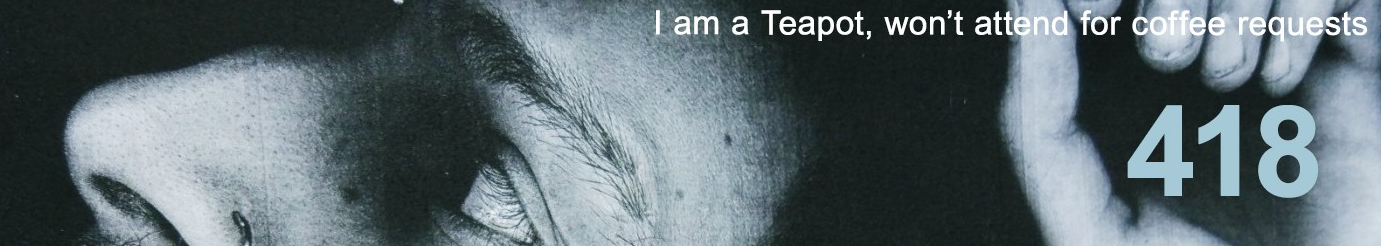
\includegraphics[width=1.15\linewidth,trim=0 0 0 34pt,clip]{assets/418-banner.png}%
  }{}%
}

\newcommand{\cvheader}{%
  \enlargethispage{3\baselineskip}%
  \color{ink}%
  \small%
  \vspace*{-4em}%
  \hspace*{-0.07\linewidth}{\transparent{0.24}\cvbanner}\par
  \vspace*{-6em}%
  {\resizebox{0.50\linewidth}{!}{\ttfamily\bfseries Dídac Llorens}}\par
  \vspace{0.26em}%
  {\resizebox{\linewidth}{!}{\ttfamily \cvHeadline \hspace{3em} Barcelona \hspace*{-1.5em}}}\par
  \vspace{0.20em}%
  {\resizebox{0.90\linewidth}{!}{\scriptsize\ttfamily
    \href{mailto:didacllorensbravo@hotmail.com}{didacllorensbravo@hotmail.com}
    \sep
    \href{https://didacll.github.io/}{Portfolio}
    \sep
    \href{https://github.com/DidacLL}{github.com/DidacLL}
    \sep
    \href{https://www.linkedin.com/in/didacllorens/}{linkedin.com/in/didacllorens}
  }}\par
  \vspace{0.42em}%
}

\newcommand{\cvBeforeEngineering}{%
  15 years in banking and insurance operations, plus formal arts/design
  training at Escola Massana, Barcelona.

  Team leadership, case triage, regulated processes, customer-facing
  problem resolution and stakeholder communication.

  Useful transfer: regulated-domain maturity, pressure, procedures,
  data quality, audit habits and responsibility for operational outcomes.
}

\newcommand{\cvMainLinks}{%
  \begin{center}
    {\resizebox{0.82\linewidth}{!}{\href{https://github.com/DidacLL}{github.com/DidacLL}}}\\[0.35em]
    {\resizebox{0.92\linewidth}{!}{\href{https://www.linkedin.com/in/didacllorens/}{linkedin.com/in/didacllorens}}}\\[0.35em]
    {\resizebox{0.86\linewidth}{!}{\href{https://didacll.github.io/}{Personal website}}}
  \end{center}
}

\newcommand{\cvEducation}{%
  \begin{tabularx}{\linewidth}{L{2.95cm} Y}
    \textbf{Universitat Oberta de Catalunya}
      & Computer Science / Software Engineering degree, Machine Learning and
        Artificial Intelligence specialization. Core university programming
        developed extensively in C, including algorithms, data structures,
        pointers and memory concepts. Expected graduation: February 2027.\\[3em]
    \textbf{IronHack}
      & Java Backend Development bootcamp including intensive production-level
        training. Capstone: IronBank microservices banking simulation.\\[3em]
    \textbf{Fundación Francisco Puerto}
      & Advanced Android application development with Kotlin.\\
    \textbf{Barcelona ITAcademy}
      & FullStack React.\\
    \textbf{PUE}
      & Linux administration -- Consorci per a la Formació Continua de Catalunya.\\
    \textbf{Escola Massana}
      & Técnico Superior en Artes Plásticas y Diseño. Formal arts/design
        training in Barcelona.\\
  \end{tabularx}%
}
